%!TEX root = ../Lab_report.tex

Next to the diffusion coefficient $D$, the electrophoretic mobility $\mu$ is an important transport coefficient of the system. It describes the motion of a polyelectrolyte chain in the presence of an external field. It is simply defined by
\begin{align}
	\mu = \frac{v}{E},
\end{align}
where $v$ is the average velocity of the polymer chain and $E$ is the applied external field. Since the system is simulated at very small time scales, it is difficult to separate the motion of the polymer that is caused by the external from diffusive motions. Therefore, an alternative definition of the electrophoretic mobility will be useful. For weak electric fields the Green-Kubo relation
\begin{align}
	\label{eq:mu}
	\mu = \frac{1}{3k_\text{B}T} \sum_{i} q_i \int_{0}^{\infty} \langle \vec{v}_i(0) \cdot \vec{v}_\text{cm}(\tau) \rangle d\tau,
\end{align}
where $i$ denotes single particles in the system (monomers and counterions) and $\vec{v}_i$ and $q_i$ their respective velocity and charge. Importantly, the mobility can also be computed from trajectories in the absence of an external electric field when using the definition given in Equation \eqref{eq:mu}.
\begin{figure}[H]
	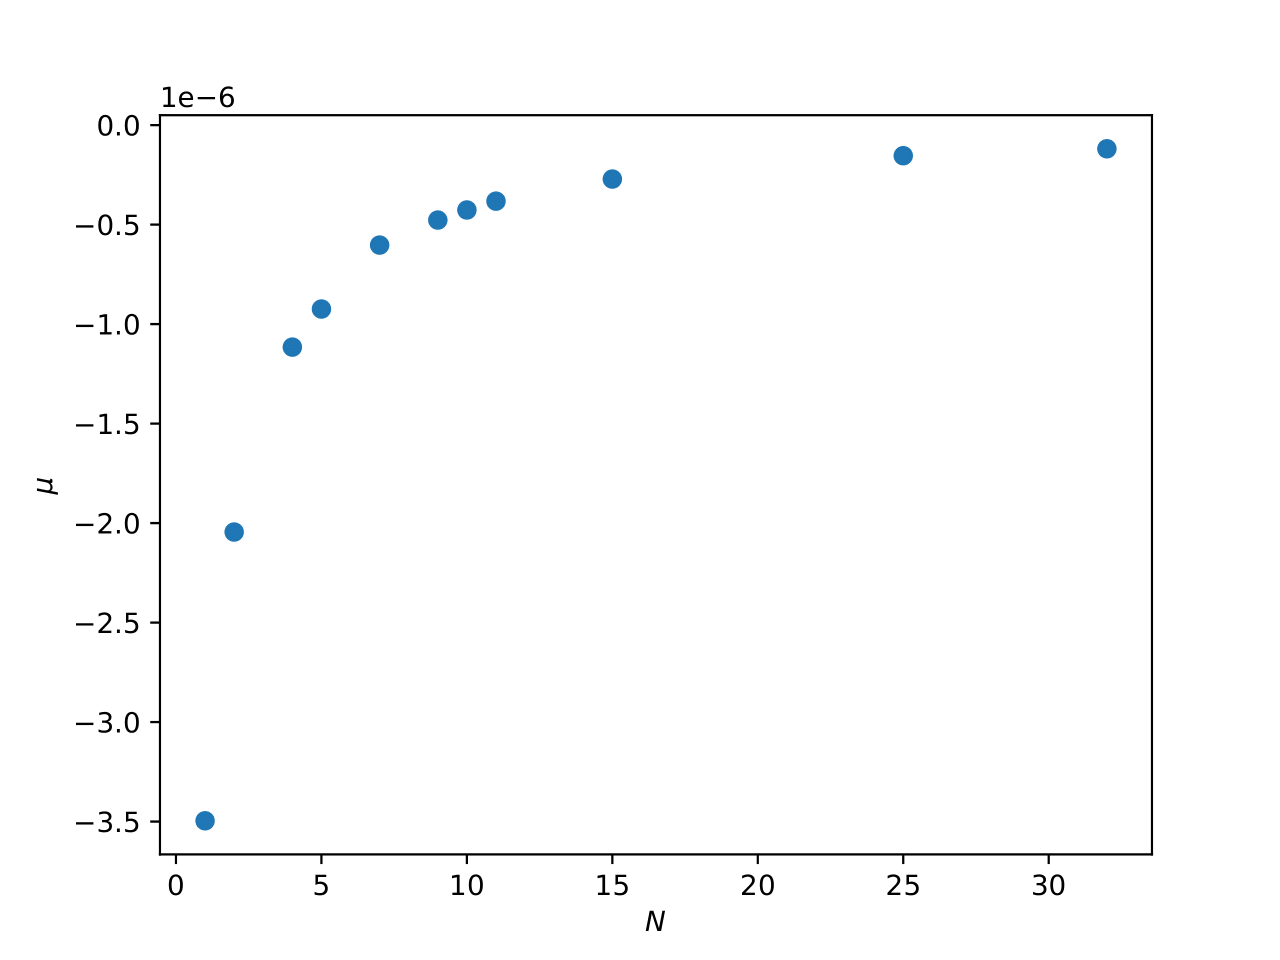
\includegraphics[width=\columnwidth]{Analysis_1/test_mobilities}
	\captionsetup{width=\columnwidth}
	\caption{Calculated mobilities of polymers as a function of chain length from MD simulations.}
	\label{fig:mobilities}
\end{figure}
The observed mobilities are in disagreement with the expected behaviour. The monotonic increase of $\mu$ with the number of monomers is only expected for short polymers. In general, in the steady state, the electric force on the polymer $\vec{F}_E = Q_\text{eff} \vec{E}$ is balanced by the counteracting solvent drag force $\vec{F}_D = -\Gamma_\text{eff} \vec{v}$. The experimentally observed constant mobility for long chains can be explained with the free draining-picture. The polymer is assumed to be penetrated by counterions, which drag along surrounding solvent. This results in the destruction of long range hydrodynamical interactions. The effective friction on the polymer scales linearly with the number of monomers for long chains, i.e.
\begin{equation}
	\Gamma_\text{eff} = \Gamma N.
\end{equation}
Together with the effective charge predicted by Manning theory of
\begin{equation}
	Q_\text{eff} = N / \xi
\end{equation}
a constant mobility
\begin{equation}
	\mu = \frac{v}{E} = \frac{Q_\text{eff}}{\Gamma_\text{eff}} = \frac{N}{\Gamma N \xi} = \frac{1}{\Gamma \xi}
\end{equation}
is obtained. In the transition region between short and long chains a mobility maximum is expected. Our results indicate an inaccurate description of hydrodynamic interaction in the system, which could be the reason for the unexpected behavior of the mobility.